\documentclass[12pt]{article}
\usepackage{fontspec}
\usepackage{fullpage}
\usepackage{hyperref}
\hypersetup{bookmarks=true,colorlinks=true,linkcolor=red,citecolor=blue,filecolor=magenta,urlcolor=cyan}
\usepackage{amsmath}
\usepackage{amssymb}
\usepackage{mathtools}
\usepackage{unicode-math}
\usepackage{tabu}
\usepackage{longtable}
\usepackage{booktabs}
\usepackage{caption}
\usepackage{enumitem}
\usepackage{graphics}
\usepackage{filecontents}
\usepackage[backend=bibtex]{biblatex}
\usepackage{url}
\setmathfont{Latin Modern Math}
\newcommand{\gt}{\ensuremath >}
\newcommand{\lt}{\ensuremath <}
\global\tabulinesep=1mm
\newlist{symbDescription}{description}{1}
\setlist[symbDescription]{noitemsep, topsep=0pt, parsep=0pt, partopsep=0pt}
\bibliography{bibfile}
\title{Software Requirements Specification for Diagnose}
\author{Andrea Clemeno}
\begin{document}
\maketitle
\tableofcontents
\newpage
\section{Reference Material}
\label{Sec:RefMat}
This section records information for easy reference.

\subsection{Table of Units}
\label{Sec:ToU}
The unit system used throughout is SI (Système International d'Unités). In addition to the basic units, several derived units are also used. For each unit, \hyperref[Table:ToU]{Tab: ToU} lists the symbol, a description and the SI name.

\begin{longtable}{l l l}
\toprule
\textbf{Symbol} & \textbf{Description} & \textbf{SI Name}
\\
\midrule
\endhead
${\text{L}}$ & volume & litre
\\
${\text{mol}}$ & amount of substance & mole
\\
${\text{s}}$ & time & second
\\
\bottomrule
\caption{Table of Units}
\label{Table:ToU}
\end{longtable}
\subsection{Table of Symbols}
\label{Sec:ToS}
The symbols used in this document are summarized in \hyperref[Table:ToS]{Tab: ToS} along with their units. Throughout the document, symbols in bold will represent vectors, and scalars otherwise. The symbols are listed in alphabetical order. For vector quantities, the units shown are for each component of the vector.

\begin{longtable}{l l l}
\toprule
\textbf{Symbol} & \textbf{Description} & \textbf{Units}
\\
\midrule
\endhead
$\mathbf{a}$ & Acceleration & $\frac{\text{m}}{\text{s}^{2}}$
\\
$C$ & Concentration & $\frac{\text{mol}}{\text{L}}$
\\
$k$ & Dimensionless constant & --
\\
$n$ & NumberV & ${\text{mol}}$
\\
$r$ & VRate & $\frac{\text{mol}}{\text{L}\text{s}}$
\\
$t$ & Time & ${\text{s}}$
\\
$V$ & Vol & ${\text{L}}$
\\
$\mathbf{v}$ & Velocity & $\frac{\text{m}}{\text{s}}$
\\
\bottomrule
\caption{Table of Symbols}
\label{Table:ToS}
\end{longtable}
\subsection{Abbreviations and Acronyms}
\label{Sec:TAbbAcc}
\begin{longtable}{l l}
\toprule
\textbf{Abbreviation} & \textbf{Full Form}
\\
\midrule
\endhead
\bottomrule
\caption{Abbreviations and Acronyms}
\label{Table:TAbbAcc}
\end{longtable}
\section{Introduction}
\label{Sec:Intro}
HIV-1 is a virus that attacks cells of the immune system needed to fight off diseases. The virus leads to an uncurable disease called AIDs. Therefore, it is useful to have a program to model these types of problems. The program documented here is called Diagnose.

The following section provides an overview of the Software Requirements Specification (SRS) for Diagnose. This section explains the purpose of this document, the scope of the requirements, the characteristics of the intended reader, and the organization of the document.

\subsection{Scope of Requirements}
\label{Sec:ReqsScope}
The scope of the requirements includes the analysis of HIV-1 concentration over time.

\section{Specific System Description}
\label{Sec:SpecSystDesc}
This section first presents the problem description, which gives a high-level view of the problem to be solved. This is followed by the solution characteristics specification, which presents the assumptions, theories, and definitions that are used.

\subsection{Problem Description}
\label{Sec:ProbDesc}
A system is needed to A system is needed to assess the risk before substantial immune destruction has occurred. The system will predict viral load at 30 days and the patient's progression.

\subsubsection{Terminology and Definitions}
\label{Sec:TermDefs}
This subsection provides a list of terms that are used in the subsequent sections and their meaning, with the purpose of reducing ambiguity and making it easier to correctly understand the requirements.

\begin{itemize}
\item{Virus: Submicroscopic parasites that infect cells.}
\item{Viral load: The concentration of HIV virus at a point in time.}
\item{Infected cells: Cells that interact with the virus replicate into cells altered by the virus.}
\item{Helper T cell: Cells of the immune system that neutralize infected cells.}
\item{Elimination: Physical quantity undergoing a decline in amount.}
\item{AIDs: Acquired Immunodeficiency Syndrome develops from an increase in HIV viral load to the extent where T cell count decreases to under 200 mol/L.}
\item{Diagnosis: The determination of a patient's condition reached by a healthcare professional.}
\item{Progression: The development towards a more advanced stage.}
\end{itemize}
\subsubsection{Physical System Description}
\label{Sec:PhysSyst}
The physical system of Diagnose, as shown in \hyperref[Figure:Virus]{Fig:Virus}, includes the following elements:

\begin{itemize}
\item[PS1:]{The HIV Virion.}
\item[PS2:]{The virus-infected cells.}
\item[PS3:]{The Helper T cell.}
\item[PS4:]{The Human Body.}
\end{itemize}
\begin{figure}
\begin{center}
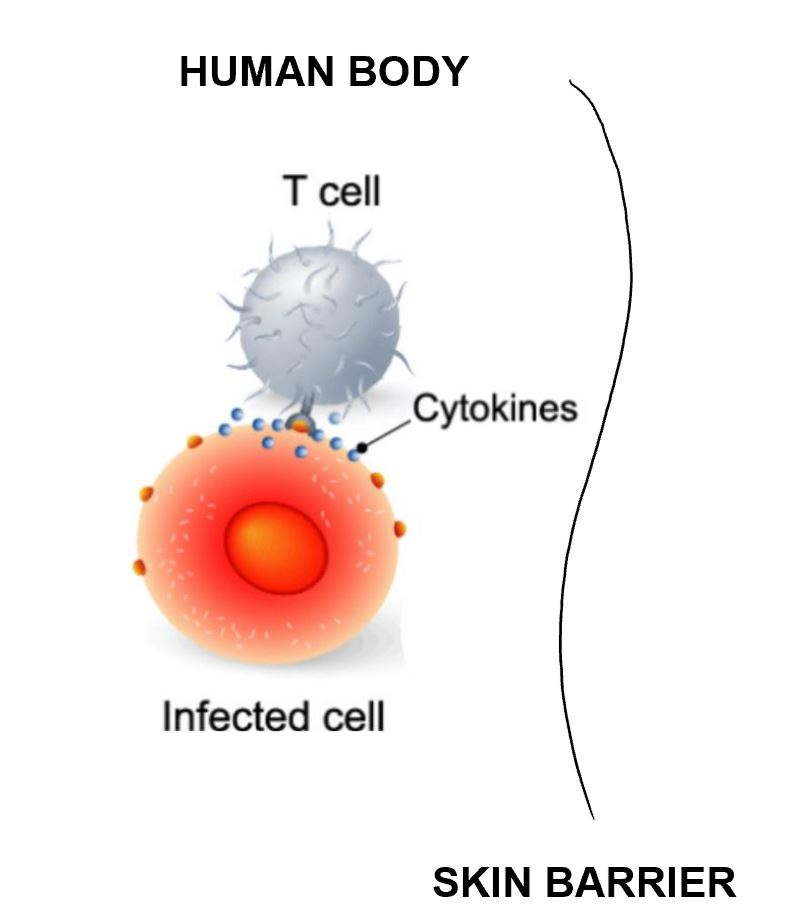
\includegraphics[width=0.7\textwidth]{../../../datafiles/Diagnose/figVirusinbody.jpg}
\caption{The physical system}
\label{Figure:Virus}
\end{center}
\end{figure}
\subsubsection{Goal Statements}
\label{Sec:GoalStmt}
Given two HIV-1 viral load datum taken on consecutive days, the goal statements are:

\begin{itemize}
\item[detElimrate:\phantomsection\label{detElimrate}]{Determine the elimination rate of the HIV Virus due to immune response.}
\item[predictVL30:\phantomsection\label{predictVL30}]{Determine the viral load at 30 days.}
\end{itemize}
\subsection{Solution Characteristics Specification}
\label{Sec:SolCharSpec}
The instance models that govern Diagnose are presented in \hyperref[Sec:IMs]{Section: Instance Models}. The information to understand the meaning of the instance models and their derivation is also presented, so that the instance models can be verified.

\subsubsection{Assumptions}
\label{Sec:Assumps}
This section simplifies the original problem and helps in developing the theoretical models by filling in the missing information for the physical system. The assumptions refine the scope by providing more detail.

\begin{itemize}
\item[initialInf:\phantomsection\label{initialInf}]{Initial infection of an HIV patient assumed.}
\item[constGrowth:\phantomsection\label{constGrowth}]{The virions will invade uninfected cells at a constant rate.}
\item[constVolume:\phantomsection\label{constVolume}]{The dimensions of the location associated with the infection remains constant.}
\item[constConditions:\phantomsection\label{constConditions}]{Temperature of the location associated with the infection remains constant.}
\item[allProductive:\phantomsection\label{allProductive}]{All infected cells are infect other cells productively.}
\item[alwaysElim:\phantomsection\label{alwaysElim}]{After viremia peak, no significant upward trends occur.}
\item[neglectDrugs:\phantomsection\label{neglectDrugs}]{The effect of drugs on the elimination rate will be not be considered.}
\item[neglectSick:\phantomsection\label{neglectSick}]{The effect of other infections on the elimination rate will be not be considered.}
\item[proportional:\phantomsection\label{proportional}]{The elimination of the virus is assumed to be proportional to the amount of viruses present.}
\end{itemize}
\subsubsection{Theoretical Models}
\label{Sec:TMs}
This section focuses on the general equations and laws that Diagnose is based on.

\vspace{\baselineskip}
\noindent
\begin{minipage}{\textwidth}
\begin{tabular}{>{\raggedright}p{0.13\textwidth}>{\raggedright\arraybackslash}p{0.82\textwidth}}
\toprule \textbf{Refname} & \textbf{TM:rate-elimination}
\phantomsection 
\label{TM:rate-elimination}
\\ \midrule \\
Label &  Average rate of elimination
        
\\ \midrule \\
Equation & \begin{displaymath}
           r=\frac{\,dA}{\,dt}
           \end{displaymath}
\\ \midrule \\
Description & \begin{symbDescription}
              \item{$r$ is the vRate ($\frac{\text{mol}}{\text{L}\text{s}}$)}
              \item{$t$ is the time (${\text{s}}$)}
              \item{$A$ is the concentration ($\frac{\text{mol}}{\text{L}}$)}
              \end{symbDescription}
\\ \midrule \\
Source & \cite{accelerationWiki} and \cite[(pg. 7)]{hibbeler2004}
         
\\ \midrule \\
RefBy & 
\\ \bottomrule
\end{tabular}
\end{minipage}
\section{Requirements}
\label{Sec:Requirements}
This section provides the functional requirements, the tasks and behaviours that the software is expected to complete, and the non-functional requirements, the qualities that the software is expected to exhibit.

\subsection{Functional Requirements}
\label{Sec:FRs}
This section provides the functional requirements, the tasks and behaviours that the software is expected to complete.

\begin{itemize}
\item[Input-Values:\phantomsection\label{inputValues}]{Input the values from \hyperref[Table:ReqInputs]{Table:ReqInputs}.}
\item[Input-Values:\phantomsection\label{inputValues}]{Input two viral load concentrations taken on  two consecutive days.}
\item[Verify-Input-Values:\phantomsection\label{verifyInput}]{The software will ensure that the inputs are not   out of bounds and in accordance with the data constraints. If any inputs are out of bounds, an error message is displayed.}
\item[Calculate-Values:\phantomsection\label{calcValues}]{Software calculates the viral load at 30 days and  the probability of progression to AIDs after 3 years.}
\item[Verify-Output:\phantomsection\label{verifyOutput}]{The output values will be cross referenced  with  the result constraints.}
\item[Output-Values:\phantomsection\label{outputValues}]{Output related requirements .}
\end{itemize}
\begin{longtable}{l l l}
\toprule
\textbf{Symbol} & \textbf{Description} & \textbf{Units}
\\
\midrule
\endhead
\bottomrule
\caption{Required Inputs following \hyperref[inputValues]{FR: Input-Values}}
\label{Table:ReqInputs}
\end{longtable}
\subsection{Non-Functional Requirements}
\label{Sec:NFRs}
This section provides the non-functional requirements, the qualities that the software is expected to exhibit.

\begin{itemize}
\item[Correctness:\phantomsection\label{correctness}]{The outputs have to adhere to the output properties in the output  constraints.}
\item[Verifiable:\phantomsection\label{verifiable}]{The code is tested with complete verification  and validation plan.}
\item[Understandable:\phantomsection\label{understandable}]{The code is modularized with complete module guide and module interface specification.}
\item[Reusable:\phantomsection\label{reusable}]{The code is modularized.}
\item[Maintainable:\phantomsection\label{maintainable}]{The traceability between requirements, assumptions, theoretical models, general definitions, data definitions, instance models, likely changes, unlikely changes, and modules is completely recorded in traceability matrices in the SRS and module guide.}
\item[Portable:\phantomsection\label{portable}]{The code is able to be run in different environments.}
\end{itemize}
\section{Likely Changes}
\label{Sec:LCs}
This section lists the likely changes to be made to the software.

\begin{itemize}
\item[Increase-time-frame:\phantomsection\label{incTimeFrame}]{The software may be expanded to cover a wide range of time frames.}
\item[More-Inputs:\phantomsection\label{moreInputs}]{The software may be expanded to include more inputs from the user  to increase the accuracy of the output.}
\item[More-Outputs:\phantomsection\label{moreOutputs}]{The software may be expanded to include more outputs  like a suggestion for therapy.}
\end{itemize}
\section{Unlikely Changes}
\label{Sec:UCs}
This section lists the unlikely changes to be made to the software.

\begin{itemize}
\item[Determine-elimination-rate:\phantomsection\label{detElimRate}]{The goal of determining the elimination rate of the virus will not likely change.}
\item[External-input:\phantomsection\label{externalInput}]{There will always be a source of input  data external to the software.}
\item[Unchanging-input-constraints:\phantomsection\label{inConstraints}]{The input constraints will not  likely change.}
\end{itemize}
\section{References}
\label{Sec:References}
\begin{filecontents*}{bibfile.bib}
@book{hibbeler2004,
author={Hibbeler, R. C.},
title={Engineering Mechanics: Dynamics},
publisher={Pearson Prentice Hall},
year={2004}}
@misc{accelerationWiki,
author={Wikipedia Contributors},
title={Acceleration},
howpublished={\url{https://en.wikipedia.org/wiki/Acceleration}},
month=jun,
year={2019}}
@misc{cartesianWiki,
author={Wikipedia Contributors},
title={Cartesian coordinate system},
howpublished={\url{https://en.wikipedia.org/wiki/Cartesian\_coordinate\_system}},
month=jun,
year={2019}}
@misc{velocityWiki,
author={Wikipedia Contributors},
title={Velocity},
howpublished={\url{https://en.wikipedia.org/wiki/Velocity}},
month=jun,
year={2019}}
\end{filecontents*}
\nocite{*}
\bibstyle{ieeetr}
\printbibliography[heading=none]
\end{document}
